
\documentclass[ms.tex]{subfiles} 
\begin{document} 

\section{Results} 
\label{sec:results} 

\begin{figure*} 
\centering 
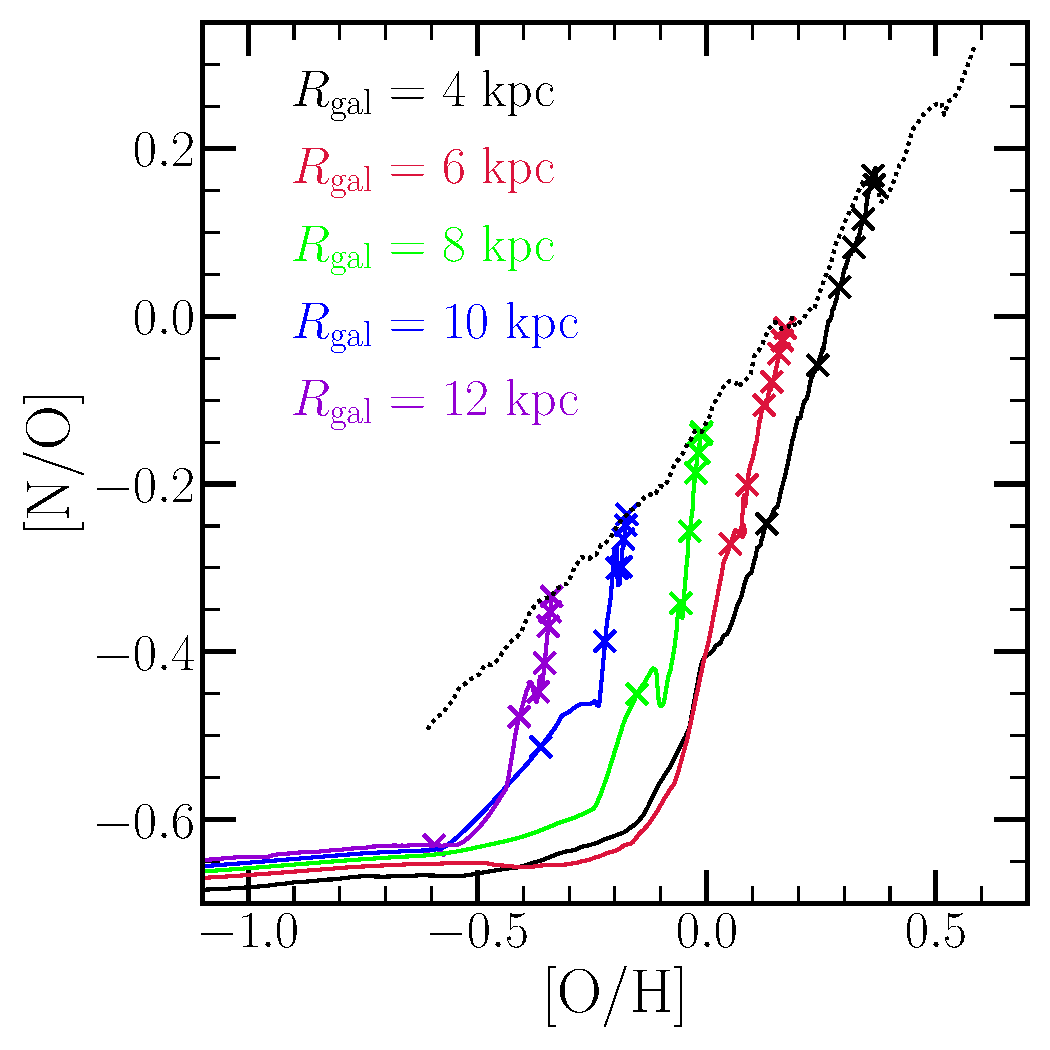
\includegraphics[scale = 0.45]{no_oh_superposition.pdf} 
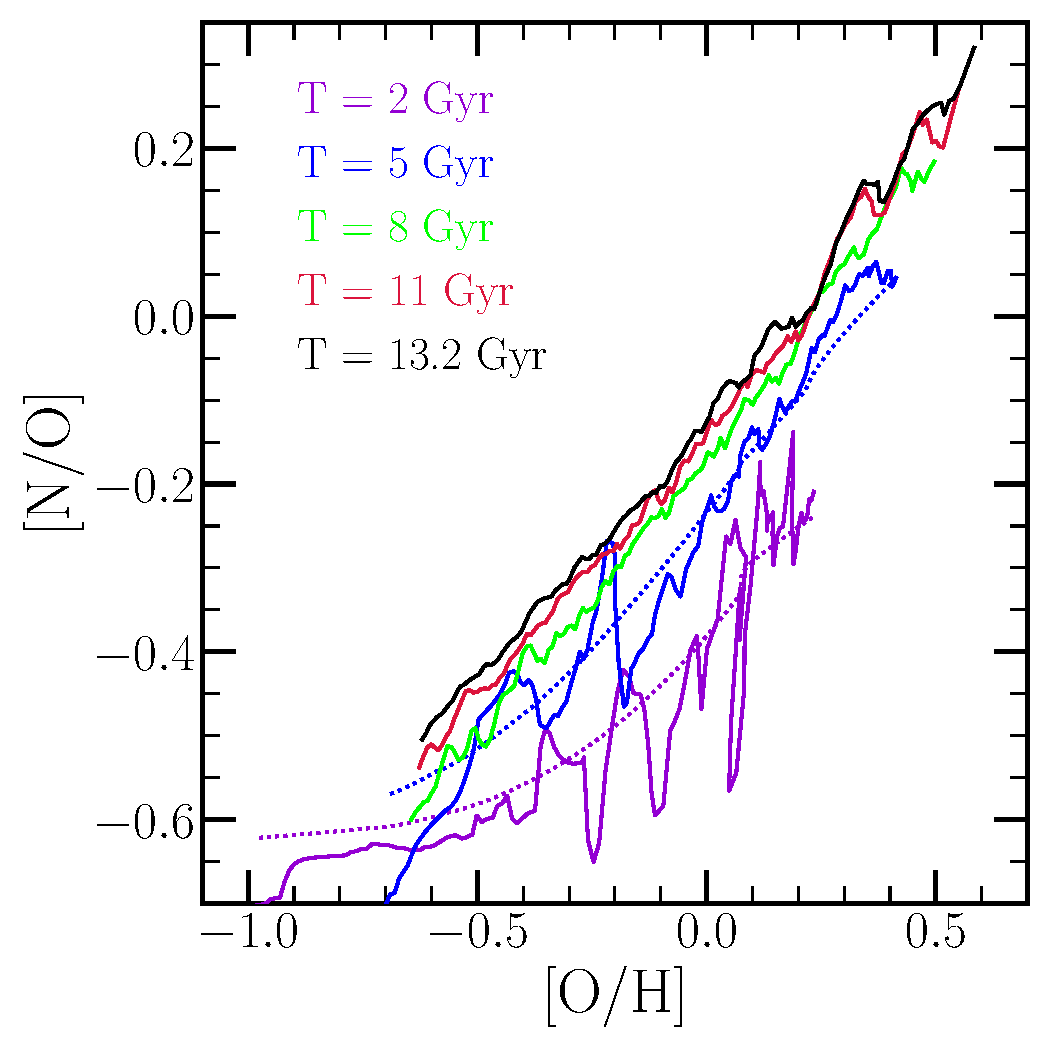
\includegraphics[scale = 0.45]{no_oh_timeevol.pdf} 
\caption{
\textbf{Left}: The gas-phase [N/O]-[O/H] relation parameterized by time at 
fixed radius (solid coloured lines) in the fiducial model. 
X's denote the abundances at~$T$ = 2, 4, 6, 8, 10, 12, and 13.2 Gyr (the 
present day) at these radii. 
The dotted blackcline is the same as the solid black line in the right panel. 
Coloured dotted lines mark the evolution of our model at~\rgal~= 10 and 12 kpc 
when stellar migration is neglected. 
\textbf{Right}: The gas-phase [N/O]-[O/H] relation parameterized by radius at 
various snapshots (solid coloured lines) in our fiducial model with 
the~\cristallo~yields. 
Similar to the left hand panel, coloured dotted lines denote the resulting 
relation at~$T$ = 2 and 5 Gyr when we neglect stellar migration. 
} 
\label{fig:no_oh_timeevol} 
\end{figure*} 

\subsection{Evolution of a Fiducial Model} 
\label{sec:results:fiducial} 

\begin{itemize} 
	\item Our fiducial model adopts, together with the supernova yields 
	of~\citet[][see discussion in~\S~\ref{sec:methods}]{Johnson2021}, 
	$y_\text{N}^\text{CC} = 3.6\times10^{-4}$ and the~\cristallo~AGB star yield 
	tables. 

	\item In the left panel of Fig.~\ref{fig:no_oh_timeevol}, we plot the 
	evolution of the N and O abundances in the gas phase in five rings at 
	a range of Galactocentric radii. 
	At early times, [O/H] is low and [N/O] reflects the ratio of the CCSN 
	yields ([N/O]~$\approx -0.7$). 
	As the Galaxy evolves, AGB stars begin enriching the ISM with their N 
	yields, and [N/O] increases. 
	Being an element produced primarily by CCSNe on short delay times, O 
	reaches an equilibrium abundance on timescales of a~$\sim$few 
	Gyr~\citep{Weinberg2017}, and consequently the metallicity gradient in 
	[O/H] is established soon after AGB stars begin producing N. 
	[N/O] then continues to increase at an approximately fixed [O/H] due to the 
	ongoing N production in AGB stars. 
	As a consequence, the gas phase tracks in the [N/O]-[O/H] plane are unique 
	from one another at different radii. 

	\item Because there is a delay between a stellar population's formation and 
	N production from its AGB stars ($\sim$250 Myr in this model; see 
	Fig.~\ref{fig:ssp}), stellar migration can occur in this time interval. 
	Although the bulk of migration occurs on longer timescales, this 
	characteristic delay time is comparable to the dynamical time of the Milky 
	Way and is thus an adequate amount of time for kinematic heating to at 
	least begin. 
	As a consequence, there may be a slight deficit or surplus of N-producing 
	AGB stars in a given ring at some time induced by stellar migration. 
	These tracks can thus move vertically in this plane in response to stars 
	moving between rings as the Galaxy evolves, entirely independent of the 
	SFH and the nucleosynthetic yields of stars that formed in any given ring. 
	We demonstrate this effect by comparing the solid blue and purple lines to 
	their dotted counterparts, which denote the tracks when we neglect stellar 
	migration entirely (i.e. the ``post-processing'' model 
	from~\citealt{Johnson2021}). 
	This is similar to what~\citet{Johnson2021} found for SN Ia enrichment of 
	Fe (see discussion in their~\S\S~3.2 and 3.4). 

	\item This panel also suggests that the [N/O]-[O/H] relation arises as a 
	superposition of endpoints rather than an evolutionary sequence. 
	Rather than each ring's track passing through a well-defined region of 
	abundance space, they instead evolve upward more or less parallel to one 
	another (modulo the effect of stellar migration). 
	This is a direct consequence of the fact that the [O/H] abundances approach 
	equilibrium quickly, and changes in the [N/O] ratio thereafter almost 
	entirely reflect changes in the N abundances; the result is an [N/O]-[O/H] 
	relation that reflects the Galaxy's metallicity gradient more so than 
	different evolutionary states. 
	Similar arguments have been made regarding the low [$\alpha$/Fe] stars in 
	the Galaxy~\citep[e.g.][]{Schoenrich2009, Sharma2020}. 

	\item In the right panel of Fig.~\ref{fig:no_oh_timeevol}, we plot the 
	gas-phase [N/O]-[O/H] relation predicted by the model at various snapshots. 
	To obtain this, we simply take the N and O abundances in the ISM at a given 
	snapshot for each~$\delta\rgal = 100$ pc ring at~$\rgal >$ 2 kpc and 
	plot them as a line. 
	The relation is generally time-independent after~$T \gtrsim 5$ Gyr, though 
	there is some evolution toward higher [N/O]. 
	We again demonstrate the impact of stellar migration by comparing the solid 
	blue and purple lines to their dotted counterparts, which quantify the 
	relation when we neglect migration. 
	This indicates that the complex features seen in the relation at all times 
	is an effect of stellar migration as discussed above. 

	\item \citet{Johnson2021} found that the SN Ia rate in this model can vary 
	by as much as a factor of~$\sim$3 at large radii ($\rgal\gtrsim 9$ kpc), 
	also as a consequence of stellar migration (see their Fig. 8 and discussion 
	in their~\S~3.4). 
	They demonstrate that this is a sufficiently large effect such that the 
	resultant stellar populations are Fe-poor enough to explain the 
	intrinsically young sub-component of the young~$\alpha$-rich stars observed 
	in the solar neighbourhood with APOGEE\footnote{
		Apache Point Observatory Galaxy Evolution 
		Experiment~\citep{Majewski2017} 
	}~\citep[see discussion in their~\S\S~3.2 and 3.4;][]{Chiappini2015, 
	Martig2015, Martig2016, Jofre2016, Yong2016, Izzard2018, SilvaAguirre2018, 
	Warfield2021}. 
	For N, the effect is much smaller ($\lesssim 0.1$ dex), but there are some 
	instances at early times where the impact of stellar migration is more 
	substantial. 
	The smaller effect on N enrichment rates can be understood from the 
	relative timescales of their production (see Fig.~\ref{fig:ssp} and 
	discussion in~\S~\ref{sec:yields:imf_agb}). 
	Produced on timescales of a~$\sim$couple hundred Myr, N yields are ejected 
	from stellar populations~$\sim$5 times faster than Fe (even faster in our 
	alternate AGB star yield models). 
	Consequently, there is much less time for stellar migration to occur within 
	the timescale of N production than there is within the timescale of Fe 
	production, and as a result, migration has only a small impact on the gas 
	phase N abundances. 
	This underscores the argument from~\citet{Johnson2021} that in order for 
	nucleosynthetic yields to migrate significant distances along with their 
	progenitor stellar populations, the timescale for production needs to be 
	at least comparable to the migration timescale. 

\end{itemize} 

\subsection{Comparison to Observed Gas Phase Trends} 
\label{sec:results:yields} 

\begin{figure*} 
\centering 
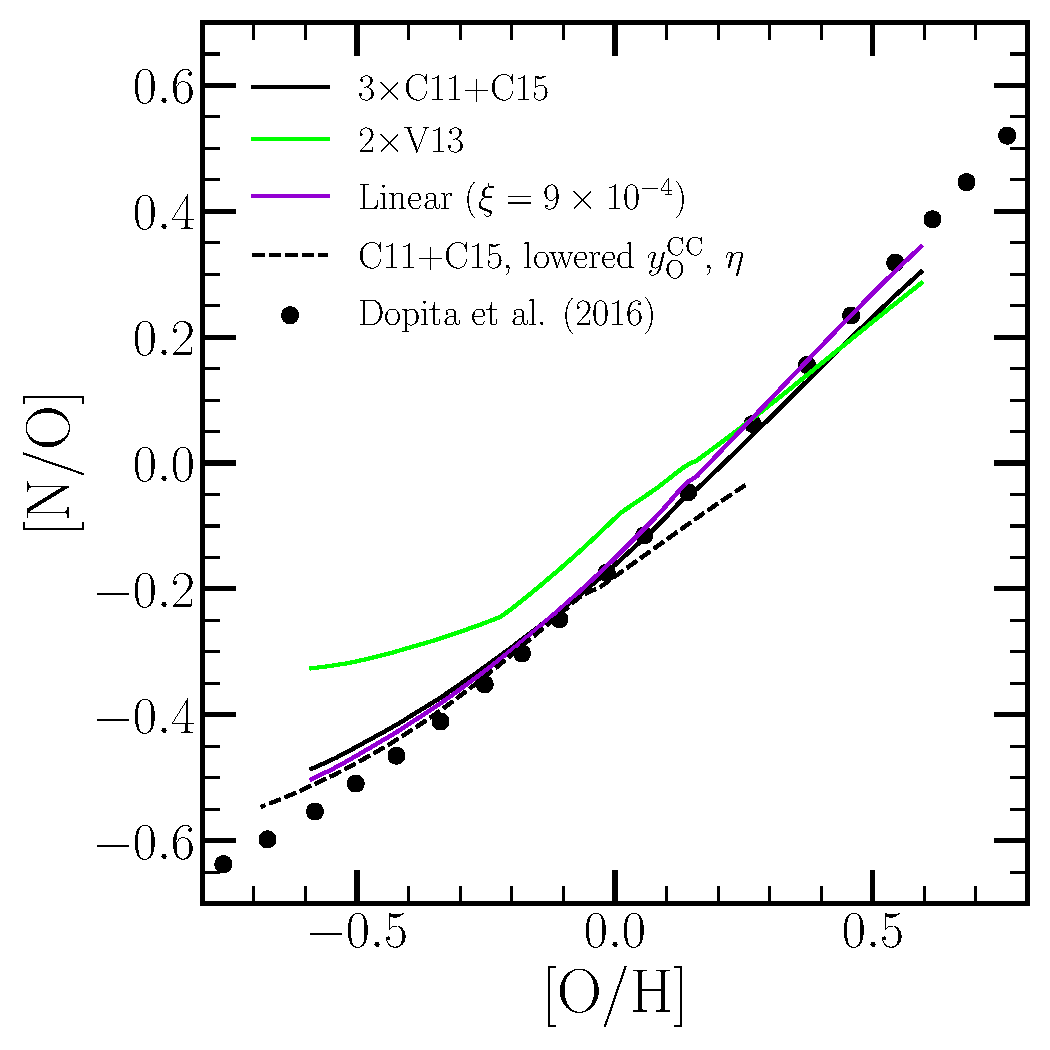
\includegraphics[scale = 0.45]{no_oh_predictions.pdf} 
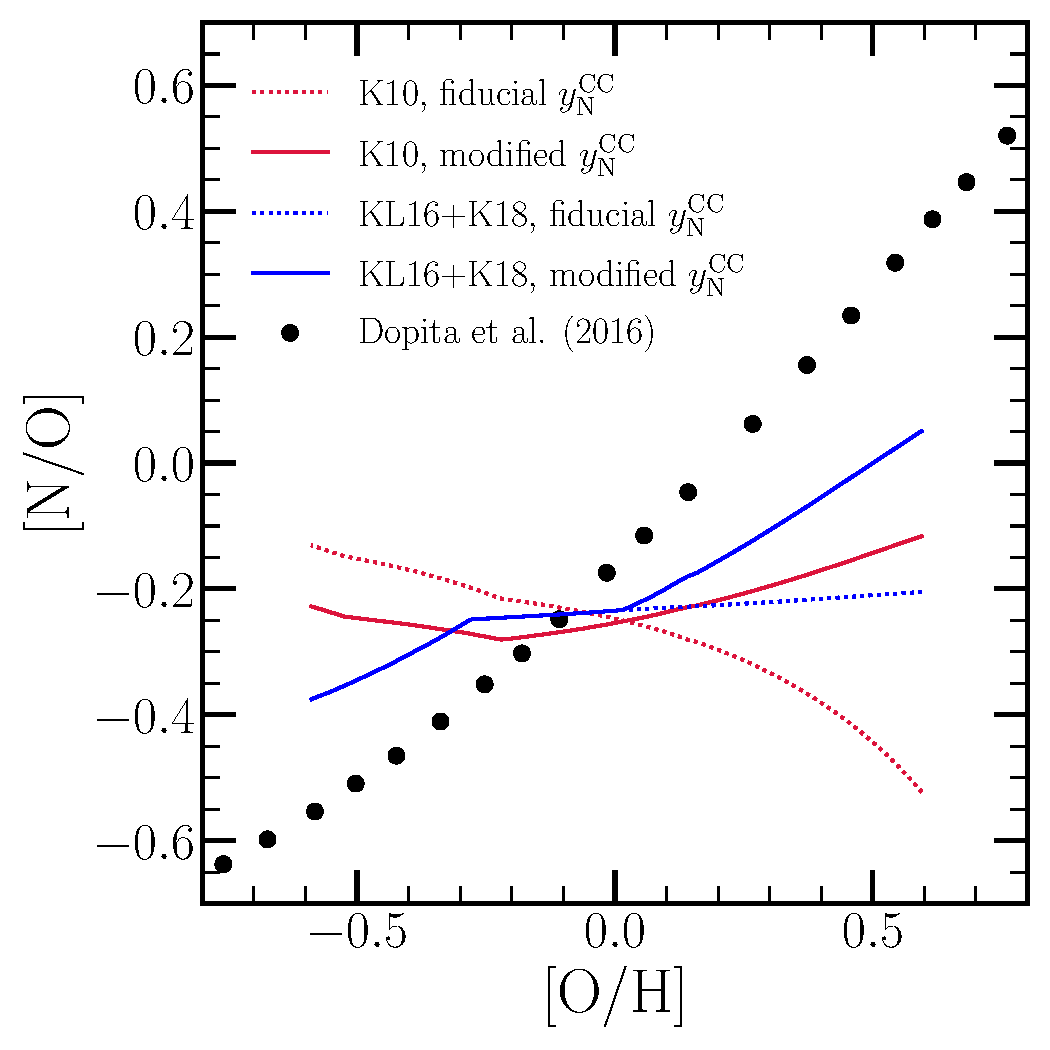
\includegraphics[scale = 0.45]{no_oh_predictions_karakas.pdf} 
\caption{
\textbf{Left}: The present day gas-phase [N/O]-[O/H] relation predicted by our 
fiducial model with each of the yield sets described 
in~\S~\ref{sec:yields:agb}. 
The~\cristallo~and~\ventura~yields are artificially amplified by factors of 
3 and 2, respectively, and we take the linear model with~$\xi = 9\times10^{-4}$. 
For observational reference, we plot the population-averaged trend for local 
stars and HII regions reported by~\citet{Dopita2016}. 
\textbf{Right}: The same as the left-hand panel, but comparing the predictions 
made by the~\karakasten~and~\karakas~yields with our fiducial value 
of~$y_\text{N}^\text{CC}$ (dotted lines, same as left-hand panel) to those with 
the alternate forms of~$y_\text{N}^\text{CC}$ (solid lines) given by equation X 
for the~\karakasten~yields and equation Y for the~\karakas~yields. 
} 
\label{fig:no_oh_predictions} 
\end{figure*} 

\begin{itemize} 
	\item We use the~\citet{Dopita2016} measurements as our observational 
	baseline. 
	They are a good representation of many results for gas phase N and O 
	abundances, and they agree well with APOGEE stellar 
	trends~\citep{Vincenzo2021}. 

	\item The left hand panel of Fig.~\ref{fig:no_oh_predictions} compares the 
	predictions of our model made with each of the AGB star yield models 
	discussed in~\S~\ref{sec:yields:agb} and visualized in 
	Fig.~\ref{fig:agb_yield_models}. 

	\item In order to successfully reproduce the observations, we find that we 
	need to artificially amplify the~\cristallo~and~\ventura~yields by factors 
	of~$\sim$3 and~$\sim$2, respectively. 
	Having originally comparing our linear model to the~\cristallo~yields in 
	Fig.~\ref{fig:agb_yield_models} with~$\xi = 3\times10^{-4}$, we amplify the 
	value of~$\xi$ by a factor of 3 here as well. 
	Although these models predict an [N/O]-[O/H] relation that is slightly 
	shallower than the~\citet{Dopita2016} measurements, the predictions are 
	reasonably within the scatter seen in Fig.~\ref{fig:no_oh_observed}. 
	{\color{red} To do: Alternatively, can this be explained by a lowering of 
	the O yields and~$\eta$, or a differential wind which preferentially 
	removes oxygen~\citep{Vincenzo2016a}}? 

	\item We are unable to reproduce the observed trend with either 
	the~\karakasten~or~\karakas~yield models. 
	\begin{itemize} 
		\item In the case of~\karakasten, the model overpredicts [N/O] at low 
		[O/H] and predicts [N/O] to~\textit{decrease} monotonically with 
		increasing [O/H]. 
		With a slope of the wrong sign, there is no multiplicative factor by 
		which we can amplify or suppress these yields in order to reproduce the 
		observations. 

		\item The~\karakas~yields improve upon the~\karakasten~predictions to 
		some extent. 
		The overprediction of [N/O] at low [O/H] is largely corrected, but it 
		predicts a relatively flat trend of [N/O] above [O/H]~$\gtrsim -0.2$, 
		leading still to an underprediction of [N/O] at high [O/H]. 
	\end{itemize} 

	\item Can an alternate parameterization of~$y_\text{N}^\text{CC}$ reproduce 
	the observations with the~\karakasten~and~\karakas~AGB star yield models? 
	\begin{itemize} 
		\item If the~\karakasten~yields are to reproduce the observations, the 
		overall N abundance must decrease at low [O/H] and increase at high 
		[O/H]; one way to do this is with a metallicity-dependent CCSN yield. 
		We therefore construct the following parameterization 
		of~$y_\text{N}^\text{CC}$: 
		\begin{equation} 
		y_\text{N}^\text{CC} = (3.6\times10^{-4})\left(\frac{Z}{Z_\odot}\right). 
		\label{eq:linear_yncc} 
		\end{equation} 
		We illustrate this model with the slanted black dotted in 
		Fig.~\ref{fig:n_cc_yields}. 
		While our fiducial model best describes the rotating CCSN models 
		of~\citet{Limongi2018}, this alternate parameterization better 
		characterizes the non-rotating models of~\citet{Limongi2018}, 
		\citet{Sukhbold2016}, \citet{Nomoto2013}, and~\citet{Woosley1995} while 
		maintaining the same base-line value of~$3.6\times10^{-4}$ at solar 
		metallicity. 

		\item If the~\karakas~yields are to reproduce the observed results, 
		then contrary to the predictions made with the~\karakasten~yields, the 
		overall N abundance at low [O/H] is fine. 
		Instead, it's only the N abundance at high [O/H] that needs 
		correcting. 
		We therefore construct a second alternate form of~$y_\text{N}^\text{CC}$ 
		by retaining the value of the fiducial yield at sub-solar metallicity 
		but assuming the value of equation~\refp{eq:linear_yncc} above solar 
		metallicity: 
		\begin{equation} 
		y_\text{N}^\text{CC} = \begin{cases} 
		3.6\times10^{-4} & (Z \leq Z_\odot) 
		\\ 
		(3.6\times10^{-4})\left(\frac{Z}{Z_\odot}\right) & (Z \geq Z_\odot). 
		\end{cases} 
		\label{eq:broken_yncc} 
		\end{equation} 

		\item We compare our model predictions with these alternate CCSN yields 
		for the~\karakasten~and~\karakas~AGB star yields in the right hand 
		panel of Fig.~\ref{fig:no_oh_predictions}. 
		These modifications were able to make up some of the difference, but 
		both models still predict an [N/O]-[O/H] relation that is simply too 
		shallow to explain the observations. 
		Although we cannot reproduce the data with either the~\karakasten~or 
		\karakas~yield models, they suffer from similar issues as 
		the~\cristallo~and~\ventura~yields. 
		\begin{itemize} 
			\item The underprediction of N yields at high metallicity is not 
			unique to~\karakasten~and~\karakas; we have to amplify 
			the~\cristallo~and~\ventura~yields by factors of a few for this 
			exact reason. 

			\item At low [O/H], the~\karakas~yields are actually the only ones 
			that can explain the observed N abundances without any 
			modification. 
			The~\karakasten~yields, however, overpredict the N abundances at 
			low metallicity. 

			\item The inverse dependence of [N/O] with [O/H] when taking 
			the~\karakasten~yields can be understood by the interaction between 
			TDU and HBB (see discussion in~\S~\ref{sec:yields:agb}). 
			Both effects are stronger at low metallicity, and since all of 
			the~\karakasten~models experiencing HBB also experience TDU (see 
			their Table 1), such a result is not surprising. 
			This is also true for the~\karakas~yields, but that model predicts 
			a relatively flat [N/O]-[O/H] relation. 
			
			\item We cannot say with any confidence based on our GCE models 
			whether or not such a wide mass range of stars should experience 
			both TDU and HBB. 
			On the one hand, this makes it difficult for the model to predict a 
			monotonic increase in [N/O] with increasing [O/H]. 
			On the other hand, such strong N production at low metallicity in 
			the~\karakas~yields is what allows them to explain the N abundances 
			at low [O/H] with no modification. 
		\end{itemize} 

		\item {\color{red} 
		We believe these results are independent of the choice of the 
		CCSN yield of O~$y_\text{O}^\text{CC}$. 
		Our value of~$y_\text{O}^\text{CC}$ = 0.015 is based on models in which 
		all stars with a ZAMS mass above 8~\msun~explode as a 
		CCSN~\citep[e.g.][]{Chieffi2013}, but the~\citet{Johnson2021} models 
		assume substantial outflows such that the equilibrium abundance 
		corresponds to a reasonable metallicity gradient within the Galaxy. 
		If we were to lower all of our CCSN yields by a factor of 3 to account 
		for failed supernovae~\citep[e.g.][]{Sukhbold2016}, then we would have 
		to also lower our mass loading factors by a factor of 3 to predict 
		similar overall abundances~\citep{Weinberg2017}. 
		Our model would thus compute similar AGB star yields for N in such a 
		scenario. 
		} 

	\end{itemize} 
\end{itemize} 

\subsection{Comparison to Stellar Abundances in the Milky Way Disc} 
\label{sec:results:vincenzo_comp} 

\begin{figure} 
\centering 
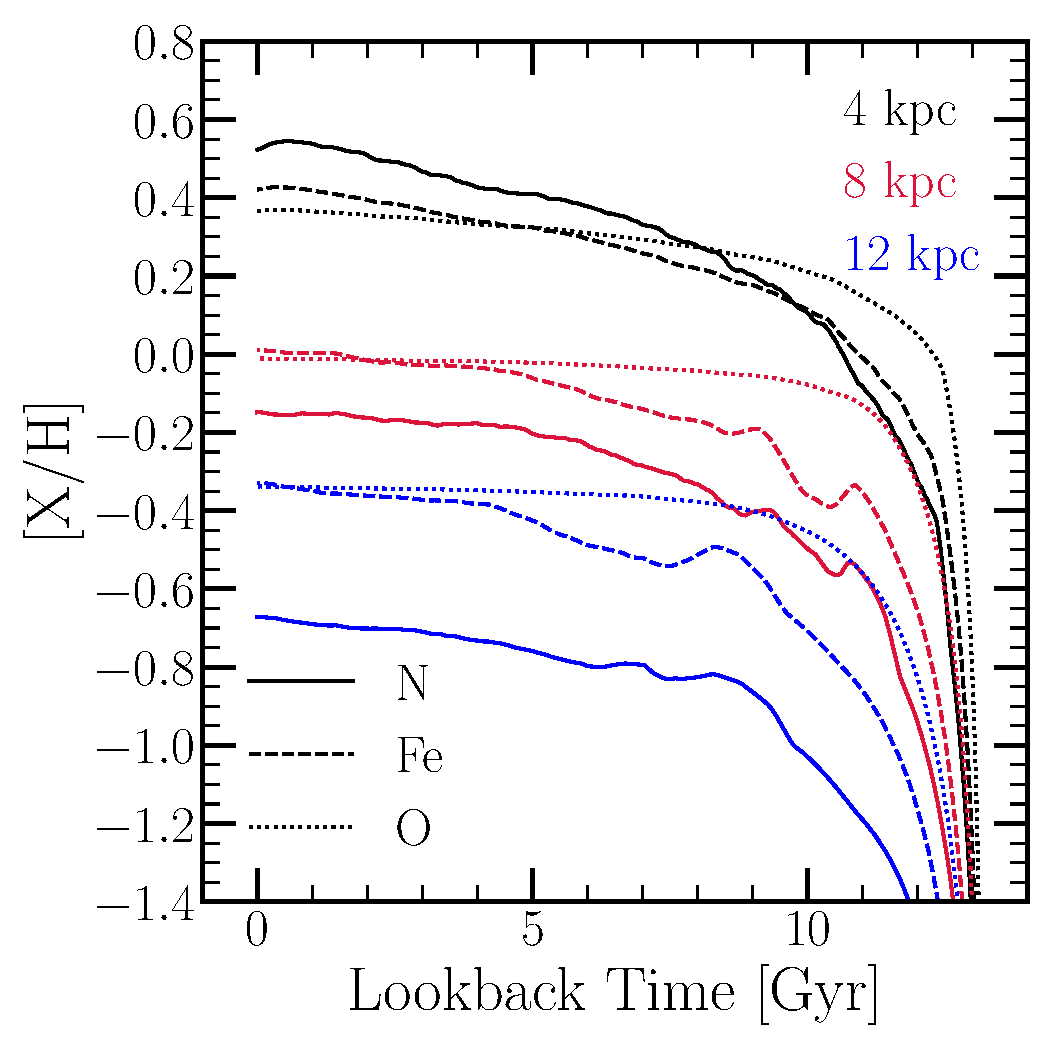
\includegraphics[scale = 0.45]{nh_feh_vs_lookback.pdf} 
\caption{
[N/H] (solid), [Fe/H] (dashed), and [O/H] (dotted) in the gas phase as a 
function of lookback time in the fiducial model at~\rgal~= 4 (black), 8 (red), 
and 12 kpc (blue). 
}
\label{fig:xh_lookback} 
\end{figure} 

\begin{figure*} 
\centering 
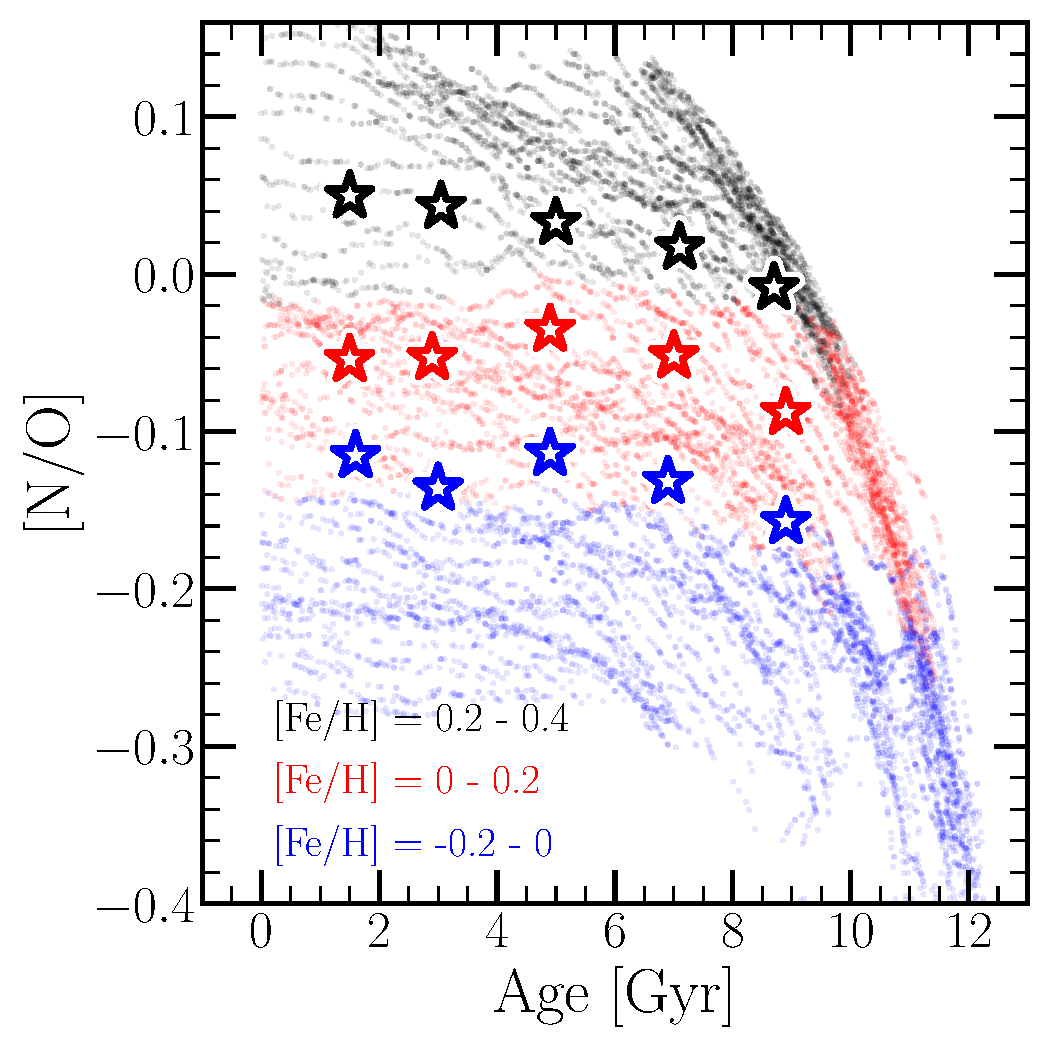
\includegraphics[scale = 0.45]{no_vs_age.pdf} 
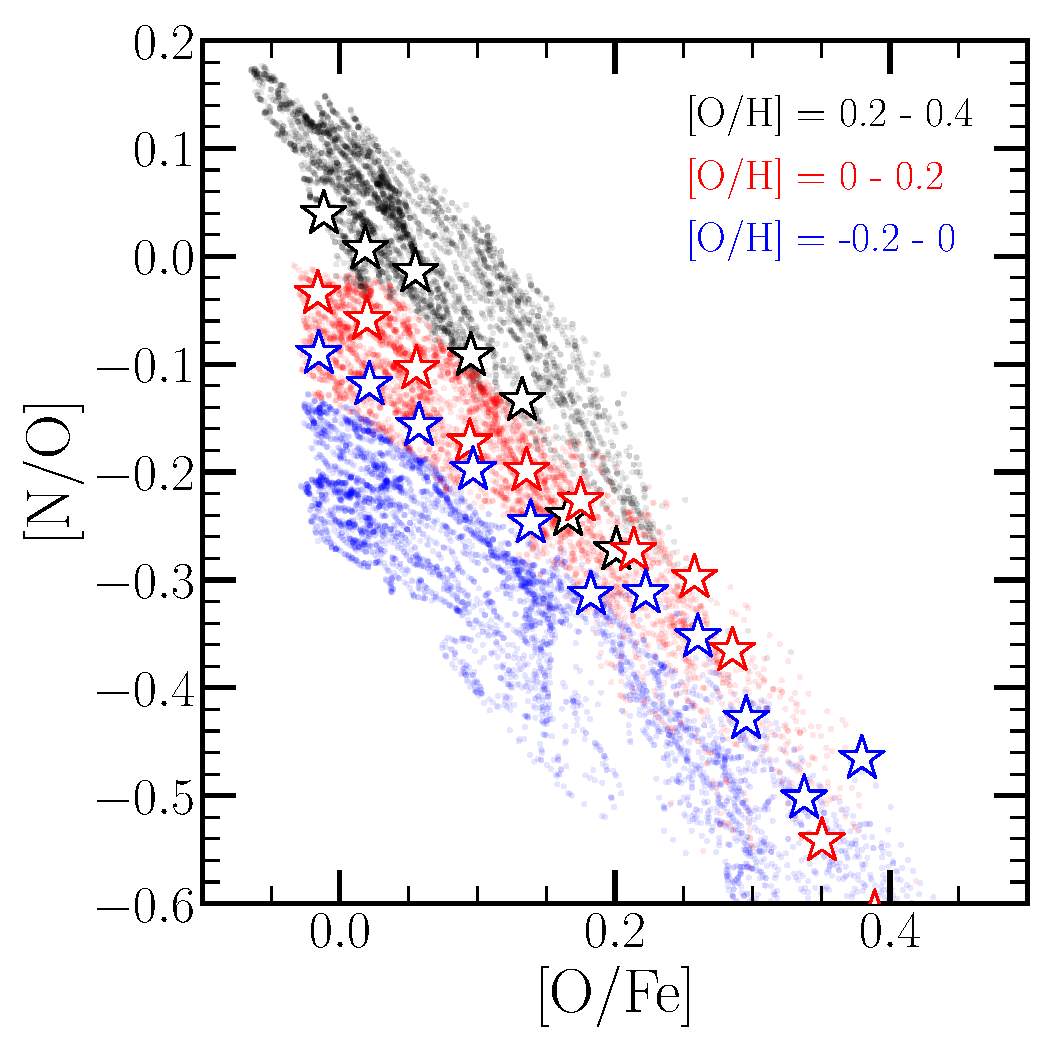
\includegraphics[scale = 0.45]{no_vs_ofe.pdf} 
\caption{
\textbf{Left}: [N/O] as a function of stellar age for 5000 stars randomly 
sampled from our model stellar populations in three bins of [Fe/H] (colored 
points). 
Stars quantify the median trend of [N/O] with age corrected for internal mixing 
in the same bins of [Fe/H] from the~\citet{Vincenzo2021} sample. 
\textbf{Middle}: The same as the left hand panel, instead showing [N/O] as a 
function of [O/Fe] in bins of [O/H]. 
} 
\label{fig:vincenzo_comp} 
\end{figure*} 

\begin{itemize} 
	\item Before comparing the predictions of GCE models to observational data, 
	it is essential that the N abundances be adjusted to account for internal 
	processes that alter the surface compositions of stars. 
	This is an important step to take before comparing GCE models to 
	observational data, because GCE models predict the birth abundances of 
	stars, and N abundances in evolved stars do not reflect their birth 
	abundance. 
	After the CNO cycle has processed much of the C and O nuclei 
	into~\Nfourteen~during a star's main sequence lifetime, this N-rich 
	material from the core is mixed with the outer convective layers, 
	increasing the N abundance in the photosphere. 
	Using~\texttt{MESA} stellar evolution models~\citep{Paxton2011, Paxton2013, 
	Paxton2015, Paxton2018} with standard mixing prescriptions, 
	\citet{Vincenzo2021} developed a prescription to approximate the birth 
	abundances of C, N, and O and apply it to a sample of APOGEE/Kepler red 
	giants. 
	They find good agreement between the APOGEE abundances and 
	the~\citet{Dopita2016} measurements, so the fiducial model's successful 
	reproduction of the~\citet{Dopita2016} trend is an indication that it also 
	successfully reproduces the overall trend of [N/O] vs. [O/H] found for 
	APOGEE disc stars. 
	In this section we focus on the stellar abundances, with which we can 
	investigate trends with age and [O/Fe]. 

	\item In Fig.~\ref{fig:xh_lookback}, we plot the evolution of the N, O, and 
	Fe abundances in the gas phase at the~\rgal~= 4, 8, and 12 kpc rings in our 
	fiducial model. 
	[N/H] is more correlated with [Fe/H] than [O/H] at all radii, and the 
	relation persists up to lookback times of~$\sim$10 Gyr. 
	This arises in part because N and Fe are both produced in significant 
	quantities by delayed enrichment sources while O is produced almost 
	entirely on short timescales by CCSNe (see discussion 
	in~\S~\ref{sec:yields}). 
	Although the production timescale of N from single stellar populations is 
	short compared to Fe (see discussion in~\S~\ref{sec:yields:imf_agb}), 
	metallicity dependent yields require more abundant species such as O and Fe 
	to be produced and reach an equilibrium before N yields stabilize. 
	When many stellar populations are present, N abundances are thus somewhat 
	limited in how fast they can increase due to the metallicity dependent 
	nature of AGB star yields;~\citet{Johnson2020} found similar results 
	regarding Fe and strontium (Sr). 
	As a consequence of its single dominant nucleosynthetic source with a 
	metallicity-independent yield, O reaches an equilibrium abundance on much 
	shorter timescales than elements like N and Fe which have significant 
	contributions from delayed sources~\citep{Weinberg2017}; because of this, 
	[O/H] is nearly independent of lookback time as far back as~$\sim$10 Gyr 
	ago while [N/H] and [Fe/H] are not. 

	\item In the left hand panel of Fig.~\ref{fig:vincenzo_comp}, we compare 
	our model predictions to their [N/O] abundances with the ages taken 
	from~\citet{Miglio2021}. 
	The model correctly predicts that the [N/O]-age relation is relatively flat 
	in bins of [Fe/H]. 
	This arises as a consequence of the N-Fe correlation described in 
	Fig.~\ref{fig:xh_lookback}: a bin in [Fe/H] is also approximately a bin in 
	[N/H], and with [O/H] more or less constant, the [N/O]-age relation at 
	fixed [Fe/H] is relatively flat up to ages of~$\sim$10 Gyr. 
	This is an important success of the model, because with uncorrected N 
	abundances, [N/O] vs. age exhibits a significant negative slope at fixed 
	[Fe/H] (see Fig. 7 of~\citealp{Vincenzo2021}). 
	Our model does, however, slightly underpredict [N/O] in the 
	[Fe/H] =~$-0.2 - 0$ bin. 
	In general, our model occupies a wider range in [N/O] at all ages than does 
	the~\citet{Vincenzo2021} measurements, suggesting that our yields scale 
	with metallicity slightly too strongly. 

	\item In the right panel of Fig.~\ref{fig:vincenzo_comp}, we compare 
	our model predicted [N/O]-[O/Fe] relation to their calculations. 
	As in the left hand panel, our model predicted stellar populations occupy a 
	wider range of [N/O] than the data, but the agreement is otherwise good. 
	The model correctly predicts that [N/O] should increase with decreasing 
	[O/Fe] at all metallicities. 
	This anti-correlation is also a direct consequence of the N-Fe correlation: 
	as the two abundances increase together in the ISM, [N/O] increases and 
	[O/Fe] decreases. 
	This is also an important success of the model;~\citet{Vincenzo2021} 
	demonstrate that when stellar N abundances are corrected for internal 
	mixing process, the dichotomy between the chemical thin and thick discs 
	persists for this element. 

	% \item We thus conclude that when a viable model for the AGB star yields 
	% of N is adopted, our GCE models are in good agreement with observed 
	% abundances of N when corrected for internal mixing processes known to 
	% affect the photospheric abundances in red giant stars. 
\end{itemize} 

\subsection{The Sources of Scatter in the [N/O]-[O/H] Relation} 
\label{sec:results:schaefer_comp} 

\begin{figure*} 
\centering 
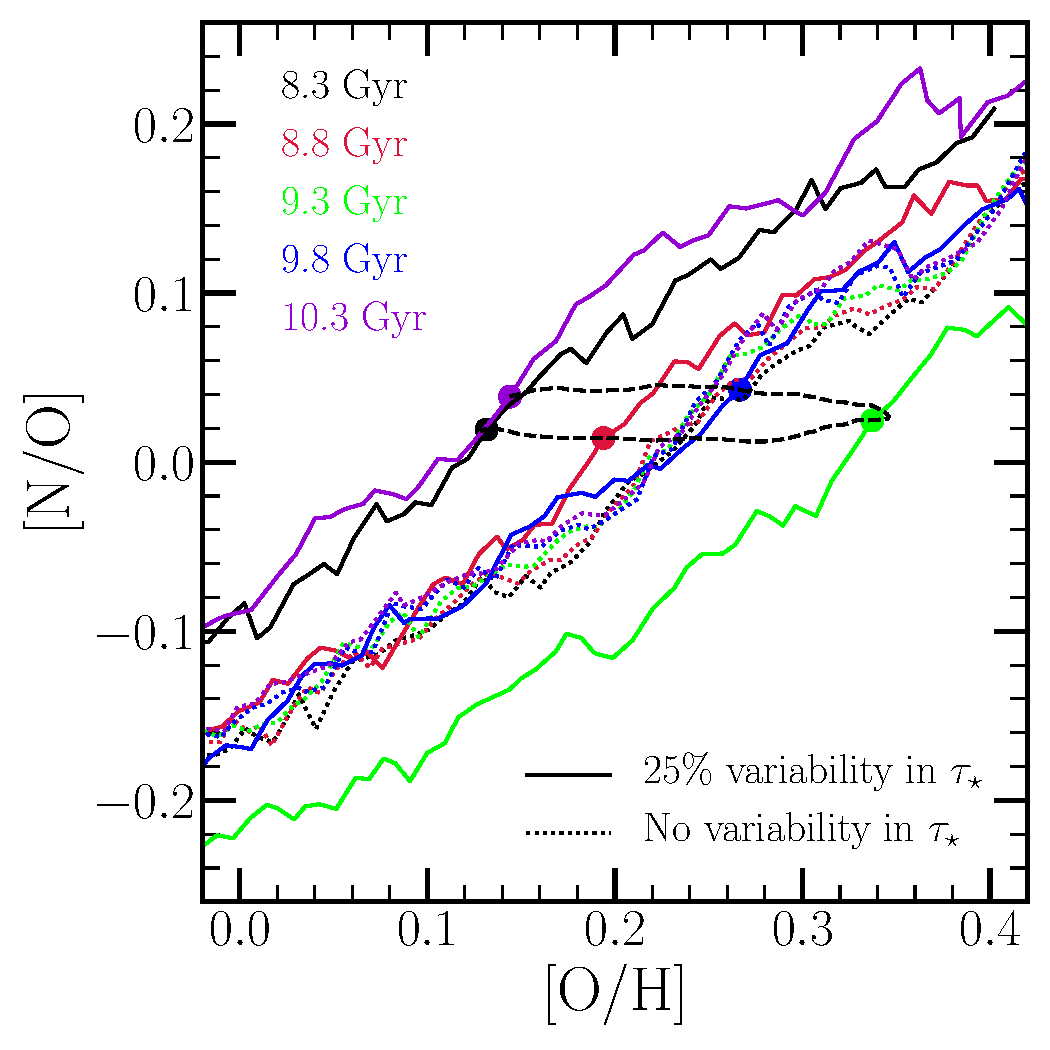
\includegraphics[scale = 0.31]{no_oh_sfevar.pdf} 
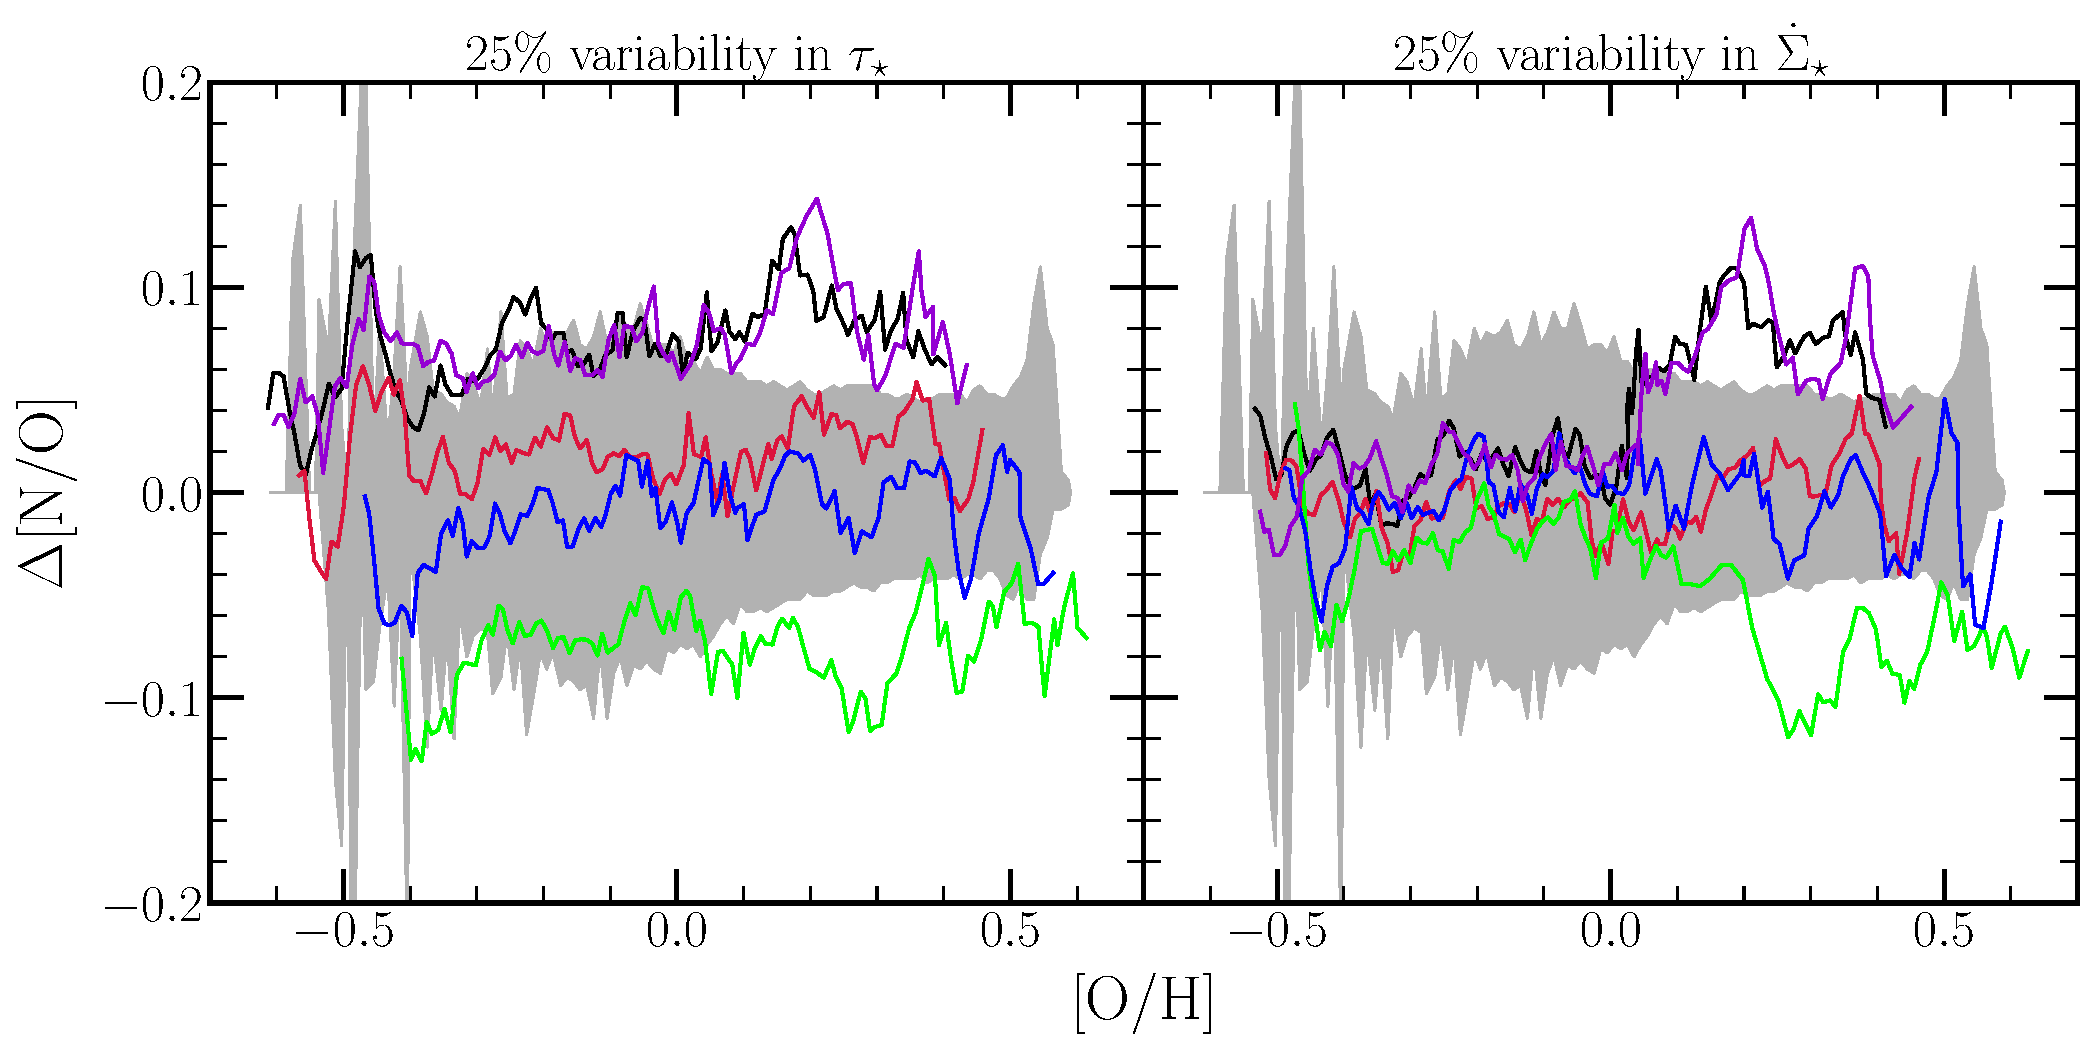
\includegraphics[scale = 0.33]{delta_no_schaefercomp.pdf} 
\caption{
\textbf{Left}: One cycle of oscillations in the [N/O]-[O/H] relation at high 
[O/H] induced by 25\% sinusoidal variability in~$\tau_\star$ (solid coloured 
lines). 
Dotted lines show the [N/O]-[O/H] relation at the same five snapshots in the 
fiducial model with no variability in~$\tau_\star$. 
The black dashed line shows the time evolution of the abundances in 
the~\rgal = 5 kpc ring, with the times of each of the five snapshots marked by 
a coloured point. 
\textbf{Middle and Right}: For the same five snapshots in the left hand panel, 
the deviation in [N/O] at fixed [O/H] relative to the fiducial model for the 
case with 25\% variability in~$\tau_\star$ (middle) and in~$\dot{\Sigma}_\star$ 
(right). 
The shaded regions in both panels quantify the width of the [N/O] distribution 
in~$10^{10.5} - 10^{11}$~\msun~galaxies in MaNGA taken 
from~\citet{Schaefer2020}. 
The median [N/O] is placed at~$\Delta$[N/O] = 0, and the lower (upper) envelope 
denotes the 16th (84th) percentile of the [N/O] distribution at a given [O/H]. 
} 
\label{fig:schaefer_comp} 
\end{figure*} 

\begin{itemize} 
	\item \citet{Schaefer2020} demonstrate that intrinsic scatter in the gas 
	phase [N/O]-[O/H] relation in MaNGA galaxies is correlated with variations 
	in the local SFE. 
	This is as expected from simple GCE models: with slower star formation, 
	more AGB stars enrich the ISM by the time it reaches a give abundance, 
	causing a higher [N/O] at fixed [O/H]. 
	However, they do not rule out radial migration as another potential source 
	of scatter in this relation. 
	Our models, taking into account the effects of radial migration on the 
	enrichment rates and thus the gas phase abundances, are the ideal tool 
	with which to address this question. 

	\item We construct two additional extensions of our fiducial model, one 
	in which the SFE exhibits 25\% sinusoidal variations in time, and the other 
	with the same 25\% variations in the SFR. 
	We modify the SFE timescale~$\tau_\star$ and SFH~$\dot{\Sigma}_\star$ from 
	the fiducial case in the following manner: 
	\begin{equation} 
	\tau_\star(\rgal, t) = \tau_{\star,\text{J21}}(\rgal, t)\left(1 + 0.25\sin 
	\left(\frac{2\pi t}{2\text{ Gyr}}\right)\right)
	\end{equation} 
	\begin{equation} 
	\dot{\Sigma}_\star(\rgal, t) = \dot{\Sigma}_{\star,\text{J21}}(\rgal, t) 
	\left(1 + 0.25\sin \left(\frac{2\pi t}{2\text{ Gyr}}\right)\right), 
	\end{equation} 
	where~$\tau_{\star,\text{J21}}$ and~$\dot{\Sigma}_{\star,\text{J21}}$ refer 
	to the SFE timescale and SFH in the fiducial model taken 
	from~\citet{Johnson2021}. 

	\item In a real galaxy, variability in the SFE and the SFR are likely 
	non-sinusoidal and not with constant amplitude. 
	However, when observing a sample of galaxies, they will have different 
	amplitudes and be seen at different phases in their variability, and the 
	impact of this on their N and O abundances will present as intrinsic 
	scatter in the inferred trend. 
	By comparing models with radial migration with and without reasonable 
	amounts of variability in these quantities will provide insight into which 
	of the two is more likely to drive scatter in the abundances. 

	\item In the left panel of Fig.~\ref{fig:schaefer_comp}, we plot the 
	predicted gas-phase [N/O]-[O/H] relation at high [O/H] for five snapshots 
	covering one cycle of the fluctuations induced by variability 
	in~$\tau_\star$. 
	This model predicts a~$\sim$0.15-dex dynamic range in [N/O] at fixed [O/H], 
	where as the model with no variability in~$\tau_\star$, denoted by the 
	dotted lines, predicts the relation to be nearly constant in comparison 
	over this time interval. 
	Because both models include the effects of stellar migration, we therefore 
	argue that reasonable variability in the local SFE is a more likely source 
	of intrinsic scatter in the gas phase [N/O]-[O/H] relation; we find 
	similar results for varability in the SFR. 

	\item Such behavior is driven by the constant tug-of-war between dilution 
	and re-enrichment associated with oscillations in~$\tau_\star$. 
	In this model,~$\dot{\Sigma}_\star$ is the same as it was 
	in~\citet{Johnson2021}, so it is not the SFR which varies but rather the 
	gas supply. 
	When the gas supply increases, the ISM becomes diluted, decreasing [O/H]. 
	Because the AGB star yields of N with our fiducial~\cristallo~model are 
	roughly linear with metallicity, the decrease in the N abundance due to the 
	now lowered yields are in direct proportion to the amount of dilution but 
	with a slight delay. 
	As a result, [N/O] is only marginally affected by the fluctuations in the 
	overall abundance. 
	The variations in the [N/O]-[O/H] relation that the model predicts are 
	therefore more of a consequence of variability in [O/H] than in [N/O]. 
	We demonstrate this with the black dashed line in the left hand panel of 
	Fig.~\ref{fig:schaefer_comp}, which traces out the evolution of the 
	abundances at~\rgal~= 5 kpc over the same time interval. 
	In general, [N/O] is affected only at the~$\sim$0.05-dex level while 
	[O/H] varies with an amplitude of~$\sim$0.25-dex. 
	As the gas supply falls off, enrichment proceeds in a gas-starved ISM, 
	which increases [O/H] once more, but [N/O] to a lesser extent for similar 
	reasons, and the cycle repeats itself. 

	\item When~$\dot{\Sigma}_\star$ varies,~$\Sigma_\text{gas}$ and 
	consequently the abundances vary instead at a value of~$\tau_\star$ that 
	varies only as much as the adopted~$\dot{\Sigma}_\star - \Sigma_\text{gas}$ 
	relation from~\citet{Johnson2021} dictates it should (see discussion in 
	\S~\ref{sec:methods}), with no additional variations in time. 

	\item In the middle and right hand panels of Fig.~\ref{fig:schaefer_comp}, 
	we plot the difference in [N/O] at fixed [O/H] between the fiducial model 
	and those with variability (i.e. the vertical offset between the solid and 
	dotted curves in the left hand panel). 
	Both scenarios produce offsets in [N/O] at high [O/H] (which as discussed 
	above are more offsets in [O/H] at fixed [N/O]), but the model with 
	variations in~$\dot{\Sigma}_\star$ does not predict any significant 
	fluctuations in the abundances at [O/H]~$\lesssim -0.2$. 
	This difference is a consequence of the mathematical form 
	of~$\tau_{\star,\text{J21}}$ (see discussion in~\S~\ref{sec:methods}) and 
	the fact that these models run~\vice~in star formation mode. 
	The low [O/H] end of this relation arises from large~\rgal~due to the 
	metallicity gradient, and the surface densities of gas our model predicts 
	at these radii are in 
	the~$\dot{\Sigma}_\star \propto \Sigma_\text{gas}^{3.6}$ portion of the 
	adopted~$\dot{\Sigma}_\star - \Sigma_\text{gas}$ relation. 
	However, since these models run from a specified SFH, it's not that the SFH 
	is a strong function of the gas supply but rather that the gas supply is a 
	weak function of the SFH. 
	As a consequence, 25\% oscillation in~$\dot{\Sigma}_\star$ therefore have 
	little impact on the ISM gas supply; there is then a minimal impact on 
	abundances since the effect of dilution is greatly minimized. 
	At smaller~\rgal~(i.e. higher [O/H]),~$\Sigma_\text{gas}$ varies more 
	strongly with~$\dot{\Sigma}_\star$, and as expected the impact on 
	abundances is more significant. 
	If we were to adopt an alternate form of 
	the~$\dot{\Sigma}_\star - \Sigma_\text{gas}$ relation, such as a purely 
	linear or single power-law formalism as in many GCE studies, then this 
	effect would be seen at all [O/H] when~$\dot{\Sigma}_\star$ oscillates. 
	Alternatively, we expect similar results if we were to run an equivalent 
	model with~\vice~in infall mode (i.e. specifying the infall history and 
	initial gas supply rather than the SFH). 

	\item The shaded regions in the left and middle panels of 
	Fig.~\ref{fig:schaefer_comp} quantify the scatter in the gas-phase 
	[N/O]-[O/H] relation inferred observationally by~\citet{Schaefer2020}. 
	Using data from Mapping nearby Galaxies at Apache Point Observatory 
	(MaNGA;~\citealp{Bundy2015}), an integral field unit survey, they measure 
	N and O abundances in 709,541 spaxels across 6,507 unique galaxies spanning 
	a stellar mass range from~$10^9 - 10^{11}$~\msun. 
	Since our model is appropriate for Milky Way mass galaxies, we focus our 
	comparison on the~$M_\star = 10^{10.5} - 10^{11}$~\msun~range, which cuts 
	our sample to 197,787 individual N and O measurements from the MaNGA IFU 
	spaxels. 
	In narrow bins of [O/H], we then compute the median [N/O] as well as the 
	16th and 84th percentiles of the [N/O] distribution. 
	Placing the median [N/O] at~$\Delta$[N/O] = 0, the shaded regions above and 
	below 0 in Fig.~\ref{fig:schaefer_comp} denote the difference between the 
	16th and 84th percentile of the distribution in each bin. 

	\item Our models with 25\% sinusoidal oscillations in~$\dot{\Sigma}_\star$ 
	and~$\tau_\star$ produce deviations in [N/O] at fixed [O/H] that are 
	comparable to the width of the distribution measured observationally. 
	Stellar migration, on the other hand, induces only small variations, as can 
	be seen in the left-hand panel of Fig.~\ref{fig:schaefer_comp}. 
	This traces back to the timescales of N production from single stellar 
	populations (see Fig.~\ref{fig:ssp} and discussion 
	in~\S~\ref{sec:yields:imf_agb}): most N production occurs quickly 
	following a stellar population's formation ($\sim$few hundred Myr), meaning 
	that most stars will not migrate far from their birth radius by the time 
	they produce their N, and the resulting impact on the gas phase abundances 
	is minimal. 

	% \item In general, galaxies will not have perfectly sinusoidal variations 
	% in their SFR or SFE, and they will also not be of a constant amplitude. 
	% Nonetheless, these models clearly demonstrate that the expected 
	% differences in N and O abundances in the gas phase is larger than that 
	% caused by radial migration as conjectured by~\citet{Schaefer2020}. 
	% Such variations will present as scatter in the gas phase abundances by 
	% observing many galaxies at different phases and with different 
	% amplitudes in their variability, which may be much more complicated 
	% that the sinusoids modeled here. 
\end{itemize} 

\end{document} 

